\documentclass[runningheads]{llncs}
\usepackage{graphicx}

\begin{document}
	\title{CS32420 Angry Blobs - Project Report}
	\author{Rhys Evans}
	\institute{Department of Computer Science,\\ Aberystwyth University, \\Aberystwyth\\
	\email{rhe24@aber.ac.uk}}
	\maketitle
	
	\begin{abstract}
		The basis of this project was to create a simple projectile launching game using three.js~\cite{ref_threejs} and physijs~\cite{ref_physijs}. The game is called 'Angry Blobs', it is a 'best of three' competition between a human player and an AI player. The two players each take a turn firing a projectile at a structure of blocks. A score is awarded each turn based on the success of the hit, at the end of the game a winner is decided based on the scores. The purpose of the project is to practically apply and demonstrate an understanding of graphics and game development techniques and principles. URLs to a working version of the game can be found below:\\\\ \url{http://users.aber.ac.uk/rhe24/angryblobs} \\ \url{http://code.rhysevans.xyz/angryblobs}\\\\ The source files provided can simply be placed into a web directory 'as-is' and it will run successfully.
	\end{abstract}
	
	\newpage
	\section{Functionalities} \label{functionalities}
	This section will briefly describe the game's key functionalities, without going into specific detail about their implementation.
	\subsection{Screens}
	There are 3 screens that are displayed throughout the game: start screen, game screen, end screen. The start screen contains a brief 'how to' for the user to understand the game, a difficulty option for the AI opponent and a start button to begin the game (see Fig.~\ref{start-screen}). The game screen contains the three.js~\cite{ref_threejs} scene and the necessary UI components (score display, round and turn display, end game button). Lastly, the end screen contains a win/lose label, a breakdown of the scores and two buttons: Home and Restart.
	\begin{figure}
		\centering
		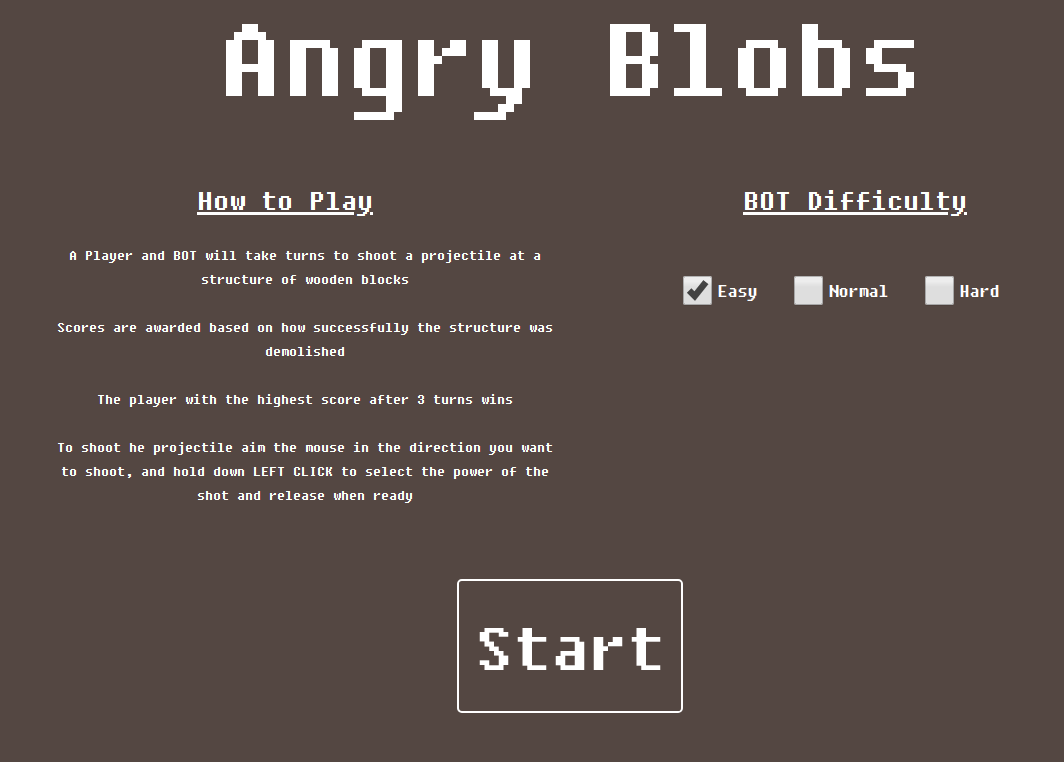
\includegraphics[width=\textwidth]{./img/start-screen.png}
		\caption{The start screen}
		\label{start-screen}
	\end{figure}
	\subsection{Firing the Projectile}\label{func_projectile}
	The projectile is fired from the left side of the scene towards the structure in a given direction at a given power. The power is decided by how long the user has held down the left mouse button for before releasing, the user is assisted by an on-screen power indicator (see Fig.~\ref{power-indicator}). There is a maximum power value that, when reached causes the power to 'loop around', meaning the user can hold down the mouse button as long as they need in order to select the correct power. 
	
	The direction in which the projectile is fired is decided by the user's cursor position, meaning the projectile is launched directly towards the cursor (ignoring the z-axis). There is an on-screen direction indicator to assist the user.
	\begin{figure}
		\centering
		
\includegraphics{./img/power-indicator.png}
		\caption{The on-screen power indicator}
		\label{power-indicator}
	\end{figure}
	\subsection{Structure Selection}
	At the start of the game, there is a full pool of pre-defined structures. At the start of each round, a random structure is selected then removed from the pool, meaning no structure can be played twice within the same game. The chosen structure for a given round is initialized twice, allowing both the Human Player and AI player to take their turn against the same structure.
	\subsection{Calculating Score}
	A score is awarded to the player at the end of their turn. The score is based on how successfully the player 'destroyed' the structure, the more individual blocks the player is able to displace, the higher their score. Scores typically range from 0-150 and a score display is updated after each turn.
	\subsection{AI Player and Difficulty}
	The AI player, known as 'BOT' within the game has two strategies for attempting to destroy the structure: aiming for the structure's center or aiming for the structure's foundation. The AI player analyses the current structure to decide which strategy to use. If the structure is tall, the AI chooses the first strategy, otherwise, it chooses the second strategy. The AI player will always attempt to apply full power to the projectile; however, in order to preserve gameplay, a set error is applied to the projectile's power and direction. 
	
	The AI player's error value is decided by the game's difficulty, which is chosen by the user at the start of the game (see Fig.~\ref{start-screen}). Each difficulty maps onto a specific error value which is then applied to all of the AI player's decisions.

	\subsection{Round and Turn Alternation}\label{turns}
	In order to give the game a progressive structure, it is broken up into 3 rounds, wherein each player takes their turn - starting with the Human Player. A new round is entered after the AI player has completed its turn. Once 3 rounds have been played the game finishes and the player is the scores and is given the option to play again or return to the start menu.
	
	\section{Design and Implementation} \label{implementation}
	This section will look in detail at the design and implementation of the functionalities outlined in Section \ref{functionalities}, along with the overall design of the system. 
	\subsection{System Architecture}
	The application implements the revealing module design pattern~\cite{ref_revealing-module-pattern}. A modular codebase is very beneficial to the game's implementation, it allows specific elements of the system to be separated, ultimately making maintenance and adaptation much easier. Implementing the revealing module pattern ~\cite{ref_revealing-module-pattern} also limits the use of the global scope and encourages good encapsulation. The application is split into 5 modules: 
	\begin{itemize}
		\item \textbf{Game} - Handles all of the game logic 
		\item \textbf{Opponent} - Handles the opponent's behaviour
		\item \textbf{Three} Components - Handles all three.js scene objects (camera, lights, meshes, textures, etc.)
		\item \textbf{UI} - Handles the UI components of the game (power indicator, score display, etc.)
		\item \textbf{User Input} - Handles all user input (button presses, mouse movement, etc.)
	\end{itemize}
	\subsection{Screens}
	A finite-state machine (see Fig.~\ref{fsm}) handles all of the game's screens, each screen is tied to a specific state; therefore, only one screen can be shown at any given time. Using a finite-state machine also means that behaviour specific to a screen can only be executed when in the associated state.
	
	The finite-state machine is implemented in the Game module using a variable to store the current state and a function to change state. Changing the state using a function, as opposed to simply changing the variable allows behaviour to be tied to state changes.
	\newpage
	\begin{figure}
		\centering
		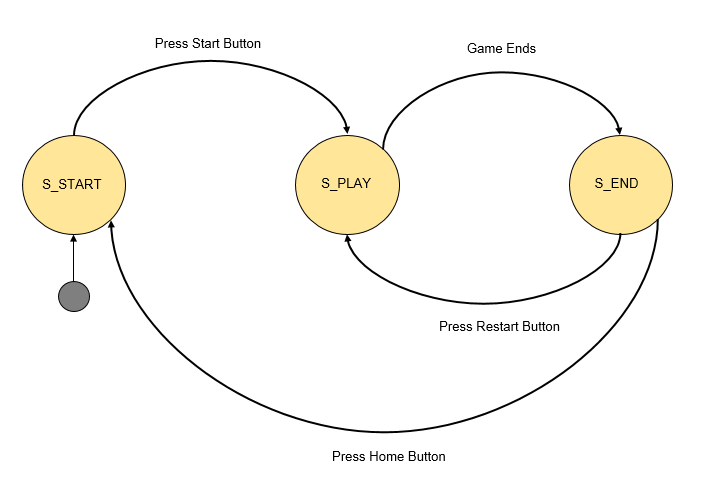
\includegraphics[width=\textwidth]{./img/fsm.png}
		\caption{The finite-state machine that handles all game screens}
		\label{fsm}
	\end{figure}
	\subsection{Firing the Projectile}
	As mentioned in~\ref{func_projectile} the projectile's direction and power is entirely based on user input. In order to accurately convert the user's cursor position into a 2D direction vector a raycaster~\cite{ref_raycast} was used. Using the raycaster allowed for cursor picking empty space, providing the threejs world co-ordinates that the cursor was currently hovering over. These co-ordinates were then inputted into a 3D vector, where the z value was always 0. This vector was used to constantly update the direction indicator.
	
	In order to allow the user to select the projectile's power in an intuitive way, the user input module measures how long the left mouse button has been held down for. This is done using jQuery's 'mouseDown' and 'mouseUp' events~\cite{ref_jquery-events}. The 'mouseDown' event begins a timer that measures how long the mouse has been pressed for and constantly updates the power value and the on-screen indicator. In order to convert milliseconds into a sensible power value within the game's range (0-50), the following formula is used:
	\begin{equation}
		power = ((currentTime - mouseHeldDownTime) / 40) \; mod \; maximumPower
	\end{equation}
	Where 40 is a constant to convert milliseconds to a sensible power value that has the modulo 50 applied to it to keep it within the 0-50 range. The number 40 was decided as it would allow the power to range from 0-50 in 2 seconds, meaning the user doesn't have to hold down the mouse for too long.
	
	Once the user releases the mouse button, the 'mouseUp' event handler stores the power the user has selected, along with the projectile's direction and calls physijs's 'applyCentralImpulse' function. This function requires a single 3D Vector as a parameter, here the direction vector is multiplied by power (a scalar value), giving both a direction and magnitude to the projectile's impulse.
	\subsection{Structure Generation}
	All of the game's structures are represented as 2D Arrays, with each element having 3 possible values: vertical, horizontal or empty (See Fig.~\ref{structure}). This allows for many different structures to be created with relative ease. For this project all structures were manually created and inputted; however, random generation could be a very interesting future implementation. Creating a structure in the threejs scene from its array representation was one of the most challenging aspects of the project. In order to keep the algorithm as simple as possible, all individual bricks are of uniform size. This means an individual brick's position relies only on its own orientation and the orientation of all bricks in the same 'column'. In order to place the structure in the right position (right of the screen), the structure is created with the first element of the array being placed at the far right of the screen. 
	\begin{figure}
		\centering
		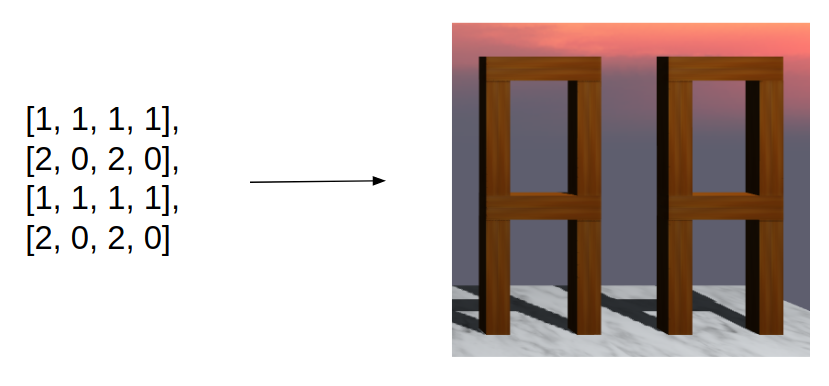
\includegraphics[width=\textwidth]{./img/structure.png}
		\caption{A structure's array representation vs in-game}
		\label{structure}
	\end{figure}
		
	\subsection{Calculating Score}
	A player's score is determined by how successfully they were able to 'destroy' a given structure. This is measured by how many individual bricks they were able to displace and by how much, each brick's distance from its original position  is added to the score. In order to normalize the score for each structure, the total score is divided by the number of bricks in the structure. This ensures that a player's possible score is not dependant on the structure.
	
	In order to ensure brick displacement is measured accurately, each brick's position is stored at the beginning of the turn. When the turn ends, the distance between each brick's initial and final position is calculated. As the game takes place on a floating platform, if a brick falls below the platform into the 'void', the y-axis of the displacement is capped at ground level (-15).
	
	Overall, this scoring system is very simple, yet effective in judging the success of a turn. However; there are a few known weaknesses that, given future work would be addressed. For example, a fully 'destroyed' tall structure is likely to yield a higher score than a shorter structure, due to the increased distance on the y-axis that a brick can fall.
	
	\subsection{AI Player}
	Implementing the AI Player was likely the most challenging aspect of the project. In the early stages of the game's development, the AI would simply fire in a random direction within a range close to the center of the screen with random power. However, it became immediately clear that the AI needed to have different approaches for different structures. The two different approaches available to the AI Player are: aim for the structure's center and aim for the structure's foundation. Although there are certainly more effective strategies and it would be beneficial to have a greater variety of strategies, this was a good compromise to keep the AI simple.
	
	In order to choose between the two available strategies, the AI player first had to evaluate the current structure to classify it as 'short' or 'tall'. A structure is tall if: it has at least 5 layers and at least 50\% of the layers contain a vertical brick. Otherwise, the structure is classified as 'short', as all structures are stored internally as arrays, evaluating the height of the structure is very trivial. 
	
	Once the AI has classified the structure it must then apply its strategy, the most challenging aspect of this is deciding the direction to aim in order to hit the structure correctly. The simplest of the two strategies is the structure's foundation. The AI simply gets the position of the first brick on the bottom layer of the structure and uses the position as it's direction. The centermost brick in the structure is the first brick in the middle layer, this is chosen by taking the number of rows in the 2D structure array, halving it and rounding down \textit{(Math.floor((structure.length - 1) / 2))}.
	
	\subsubsection{Accounting for Gravity}
	As the desired direction of the AI's projectile is simply a 3D position within the scene, there is no guarantee that is where the projectile will land, due to the effects of gravity on projectile motion. A human player can intuitively predict these effects and alter their cursor position accordingly, however, the AI player has no such capabilities. Therefore the direction (or launch angle) of the projectile must be altered to account for these effects. The below equation can be applied to calculate the ideal launch angle in order to hit a specific point~\cite{ref_projectile-motion}, where x and y is the target position and v is the initial velocity of the projectile. 
	
	\begin{equation}
		\theta = \arctan\Bigg(\frac{v^2 \pm \sqrt{v^4 - g(gx^2+2yv^2)}}{gx}\Bigg)
	\end{equation}
	
	This equation assumes that the origin of the projectile is (0, 0). However, this isn't the case in the scene, therefore the x and y values inserted must be altered to account for the projectile's origin. Because the projectile has not yet been fired, its initial velocity is unknown. However, because of the intended impulse of the projectile is known (original direction vector multiplied by the power), the change velocity can be 'predicted' using the below equation:
	
	\begin{equation}
		\Delta v = \frac{Impulse}{mass}
	\end{equation}
	
	\textit{It should be noted that the initial velocity calculated is not 100\% mathematically correct, but is accurate enough to serve the purpose required and looks correct in-game}. Once the optimum launch angle has been calculated it can be converted to a 3D vector and used as the intended direction of the projectile.
	
	\subsubsection{Difficulty and Error}
	
	The AI player will always attempt to apply maximum power; however, as this would likely lead to very high scores in most turns an error must be applied. The error value is decided by the difficulty that the user selected in the start screen (see Fig.~\ref{start-screen}). For example, if the user selected 'normal' the AI player will have a potential error of up to 50\%. This means that the AI's desired value for both power and direction can be skewed by up to 50\% of the value. For example, as the desired power is always 50, with a potential error of 50\% the actual power can be any random value between 25 and 50. With regards to the direction, the y value is altered depending on the error (see Fig.~\ref{direction-error}). For an error of 50\%, the y value of the desired direction can be any value between:
	\begin{equation}
	y = y - y * 25\% \; and \; y = y + y * 25\% 
	\end{equation}
	
	\newpage
	\begin{figure}
		\centering
		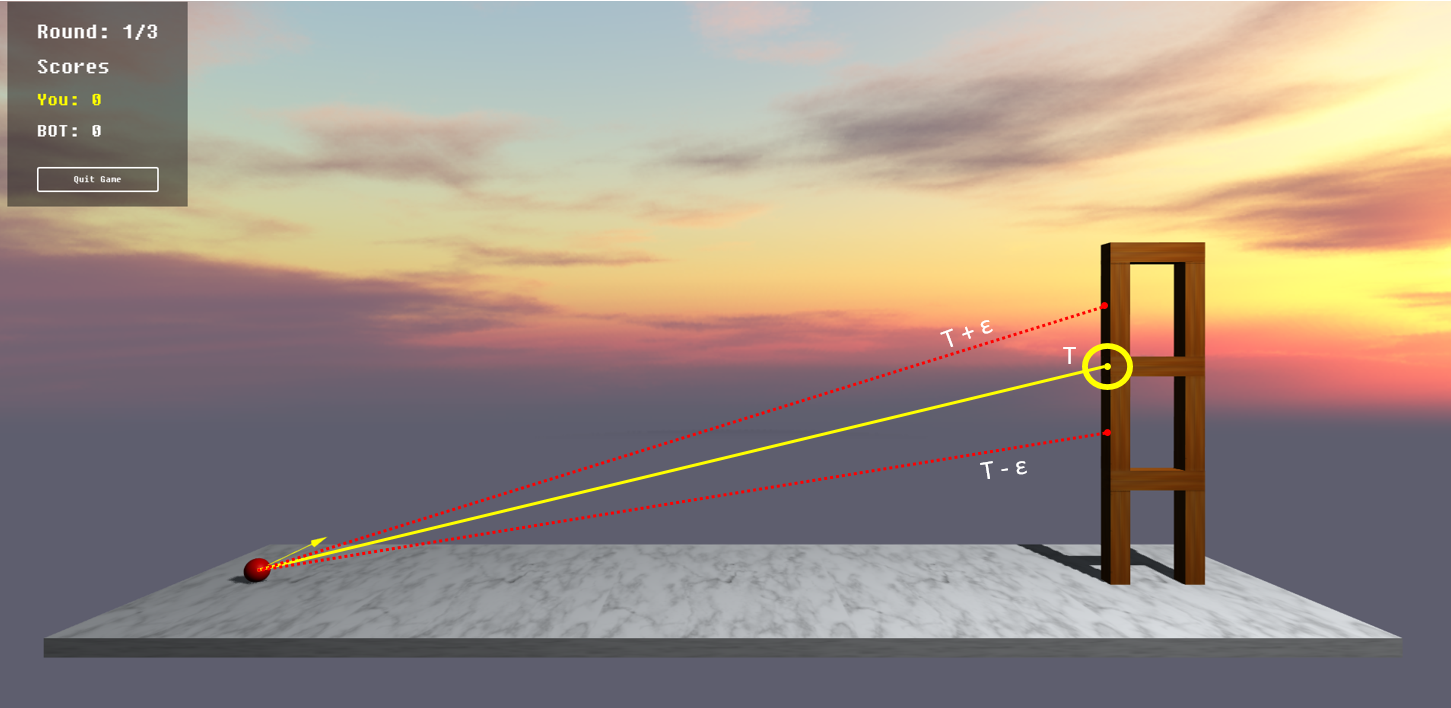
\includegraphics[width=\textwidth]{./img/direction-error.png}
		\caption{An illustration of the error applied to the AI's firing direction}
		\label{direction-error}
	\end{figure} 
	
	\subsection{Round and Turn Alternation}
	As mentioned in~\ref{turns}, a game lasts 3 rounds and each round consists of a single turn per player. Implementing the round cycle was fairly trivial, the game module has a variable to store the current round number, which is incremented after each of the AI Player's turns (as they always go last). When the round number has been incremented, the scene setup is slightly altered in order to generate a new structure.
	
	Implementing the enforcement of turn alternations proved to be more complex than initially anticipated. In the early versions of the game, turns lasted a number of seconds then were automatically alternated. However, this wasn't very robust as it would lead to turns ending prematurely and negatively impacting a player's score. Therefore there are several conditions that can be met in order for a turn to end (see Fig.~\ref{turn-flowchart}). In addition to the specific conditions, there is a 'catch-all' condition that ensures no turn can last longer than 20 seconds, this is to ensure that every turn ends and that the user isn't forced to wait around too long for the next turn.
	
	In order to properly evaluate the conditions seen in Fig.~\ref{turn-flowchart}, collision detection between the projectile and the structure had to be implemented. This was fairly trivial to implement, there is a collision handling function in the game module that is tied to the projectile object when it is created. This function evaluates what the projectile has collided with and sets a boolean variable to true. 
	
	\newpage
	\begin{figure}
		\centering
		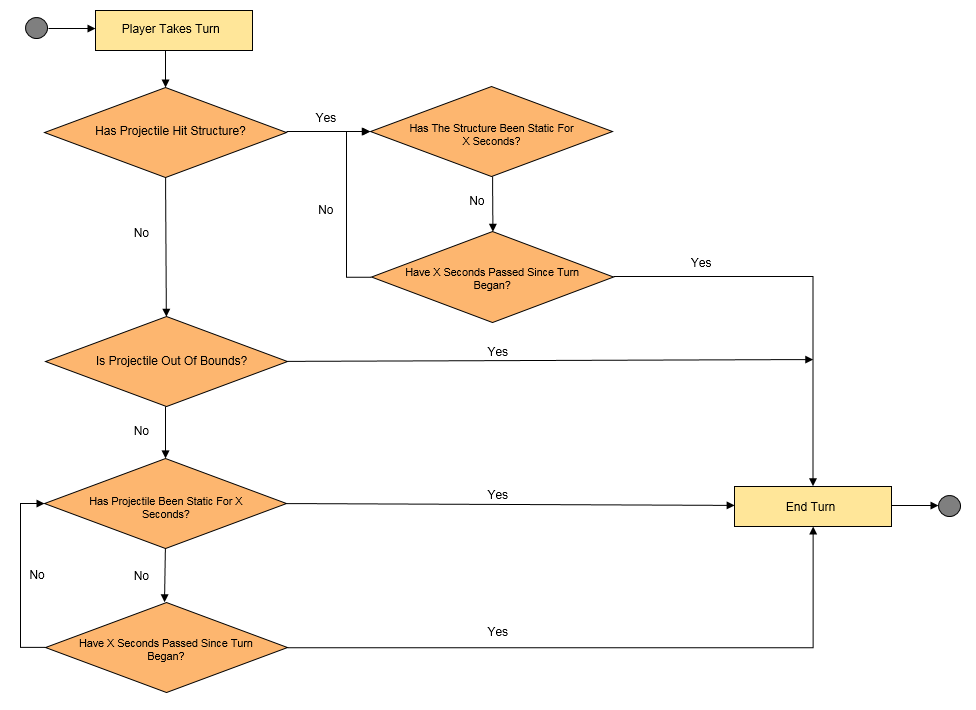
\includegraphics[width=\textwidth]{./img/turn-flowchart.png}
		\caption{A flowchart illustrating the conditions that must be met for a turn to end}
		\label{turn-flowchart}
	\end{figure} 
	
	\section{Look and Feel}
	To give the game scene a pleasant look and feel, textures were applied to both the structure~\cite{ref_wood} and the ground~\cite{ref_marble}. Textures were also used to make up the skybox around the scene~\cite{ref_skybox}, although not visible from the current camera angle, the skybox covers the entire background of the scene. In order to improve performance, all the textures used were resized to be powers of 2. The scene contains two lights, a very dim hemisphere light above the scene to give the indication of faint ambient sunlight and a bright point light behind the camera to the right. The point light casts shadows onto the scene and gives it a realistic feel, it is also positioned accurately relative to the scene's skybox.
	
	For the game's UI elements and various screens, a basic style guide was followed to retain consistency throughout the application (see Fig.\ref{styleguide}).
	
	\newpage
	\begin{figure}
		\centering
		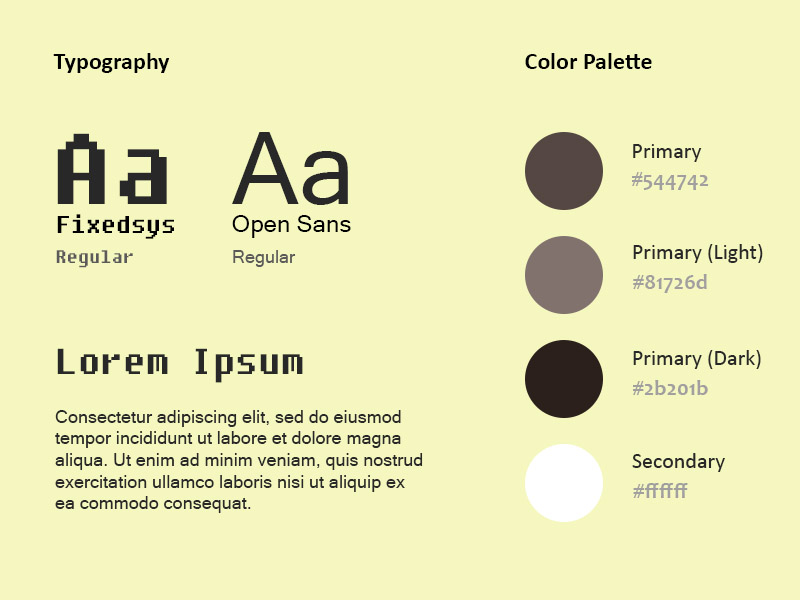
\includegraphics[width=\textwidth]{./img/styleguide.jpg}
		\caption{The application's styleguide}
		\label{styleguide}
	\end{figure}
	
	\newpage
	\begin{thebibliography}{8}
		\bibitem{ref_threejs}
		Threejs Homepage, https://threejs.org/. Last accessed 15 Nov 2018
		\bibitem{ref_physijs}
		Physijs Project Page, http://chandlerprall.github.io/Physijs/. Last accessed 15 Nov 2018
		\bibitem{ref_revealing-module-pattern}
		Chris Heilmann's Revealing Module Pattern Blog Post, https://christianheilmann.com/2007/08/22/again-with-the-module-pattern-reveal-something-to-the-world/. Last accessed 15 Nov 2018
		\bibitem{ref_raycast}
		Threejs Raycast Documentation, https://threejs.org/docs/\#api/en/core/Raycaster. Last accessed 15 Nov 2018
		\bibitem{ref_jquery-events}
		W3Schools' documentation on jQuery's Events, https://www.w3schools.com/jquery/jquery\_events.asp. Last accessed 15 Nov 2018
		\bibitem{ref_projectile-motion}
		Wikipedia Page on Projectile Motion, https://en.wikipedia.org/wiki/Projectile\_motion. Last accessed 10 Nov 2018
		\bibitem{ref_marble}
		Source of the marble texture used, https://pixabay.com/en/white-background-pattern-tile-2398946/. Last accessed 13 Nov 2018
		\bibitem{ref_wood}
		Source of the wooden texture used, https://freestocktextures.com/texture/closeup-wood-grain-plank,315.html. Last accessed 13 Nov 2018
		\bibitem{ref_skybox}
		Source of the skybox textures used, https://reije081.home.xs4all.nl/skyboxes/. Last accessed 13 Nov 2018
		
	\end{thebibliography}
\end{document}